\documentclass[tikz,border=3mm]{standalone}
\usetikzlibrary{shapes.geometric,positioning}

\begin{document}
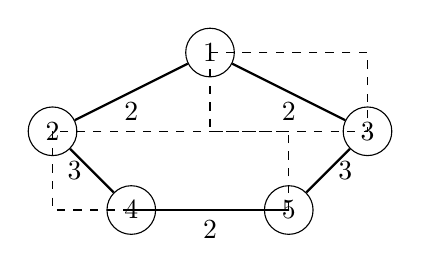
\begin{tikzpicture}[node distance=2cm]
    % Vertices
    \node[circle,draw,fill=white] (v1) at (0,0) {1};
    \node[circle,draw,fill=white] (v2) at (-2,-1) {2};
    \node[circle,draw,fill=white] (v3) at (2,-1) {3};
    \node[circle,draw,fill=white] (v4) at (-1,-2) {4};
    \node[circle,draw,fill=white] (v5) at (1,-2) {5};

    % Edges with labels
    \draw[thick] (v1) -- node[midway,below] {2} (v2);
    \draw[thick] (v1) -- node[midway,below] {2} (v3);
    \draw[thick] (v2) -- node[midway,left] {3} (v4);
    \draw[thick] (v3) -- node[midway,right] {3} (v5);
    \draw[thick] (v4) -- node[midway,below] {2} (v5);

    % Facets
    \draw[dashed] (v1) rectangle (v3);
    \draw[dashed] (v2) rectangle (v5);
    \draw[dashed] (v4) rectangle (v5);
\end{tikzpicture}
\end{document}